\documentclass[12pt]{beamer}

\usepackage{graphicx}
% \usepackage{subcaption}

\mode<presentation>
{
  \usetheme[page numbers]{Singapore}
  \setbeamertemplate{navigation symbols}{}%remove navigation symbols
  \setbeamertemplate{footline}[frame number]
  % \setbeamertemplate{page number in head/foot}[appendixframenumber]
}

\newcommand{\backupbegin}{
   \newcounter{finalframe}
   \setcounter{finalframe}{\value{framenumber}}
}
\newcommand{\backupend}{
   \setcounter{framenumber}{\value{finalframe}}
}

\usepackage[english]{babel}
\usepackage{amsmath}
\usefonttheme[onlymath]{serif}
\hypersetup{
  unicode=true,
  pdftitle={Robotics Project Proposal},
  pdfsubject={Drowbot (tentative)},
  pdfauthor={Micky Faas, Koen Putman},
  colorlinks=false,
  breaklinks=true
}

\title[ Drowbot] % (optional, use only with long paper titles)
{
\includegraphics{images/logo-01.png} }

\author[Micky Faas, Koen Putman]{Micky Faas, Koen Putman}

\institute[] % (optional, but mostly needed)
{ Leiden University - LIACS }

\date{March 15, 2018}

\begin{document}


\frame{\titlepage}
\begin{frame}[c]\frametitle{Research question}
\large
Can we automate repetitive, tedious or precise tasks in hand-made artwork using some kind of robot?
Can we do this is such a way that this robot actually takes part in the creation process instead of being just a dumb plotting device?
\end{frame}

\begin{frame}[c]\frametitle{In The Distance}
\begin{figure}
  \centering
  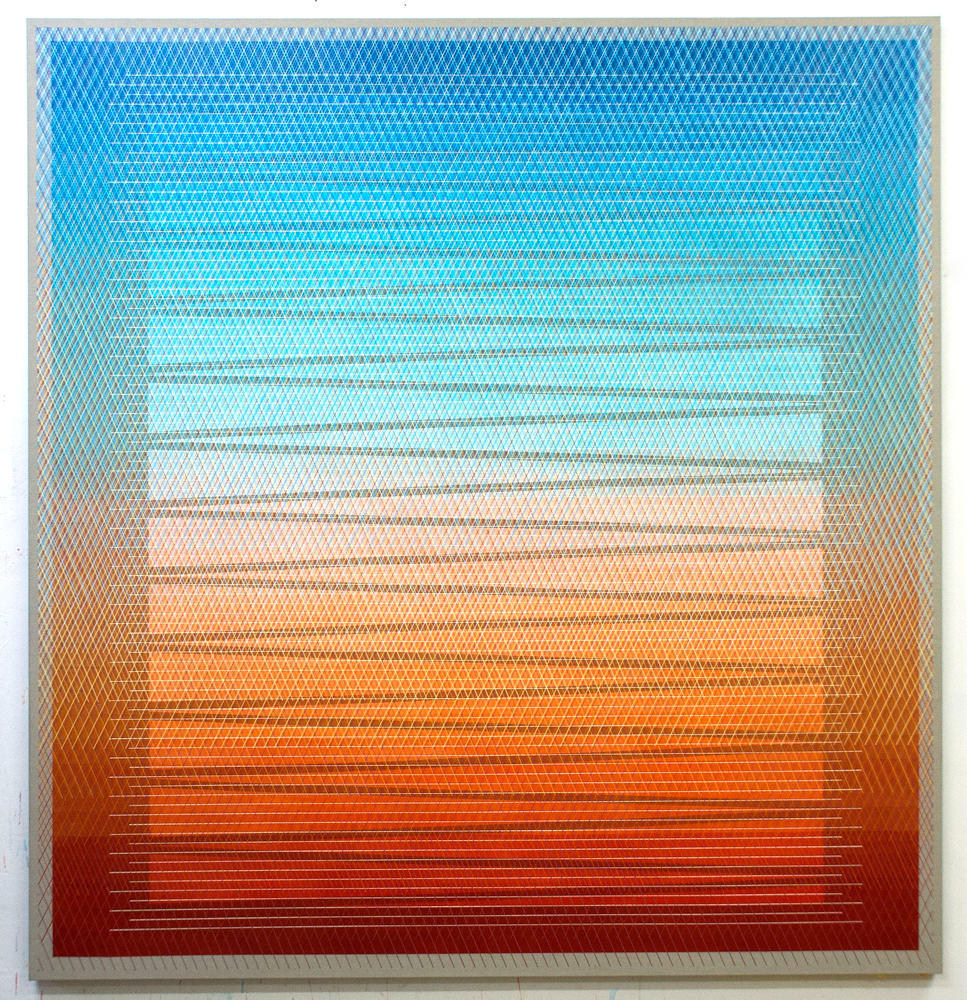
\includegraphics[width=.6\textwidth]{images/inthedistance.jpg}
  \caption{Daniel Mullen. 200x190, Acrylic on canvas, 2018}
\end{figure}
\end{frame}

\begin{frame}[c]\frametitle{1D Continuous Cellular Automaton}
\begin{figure}
  \centering
  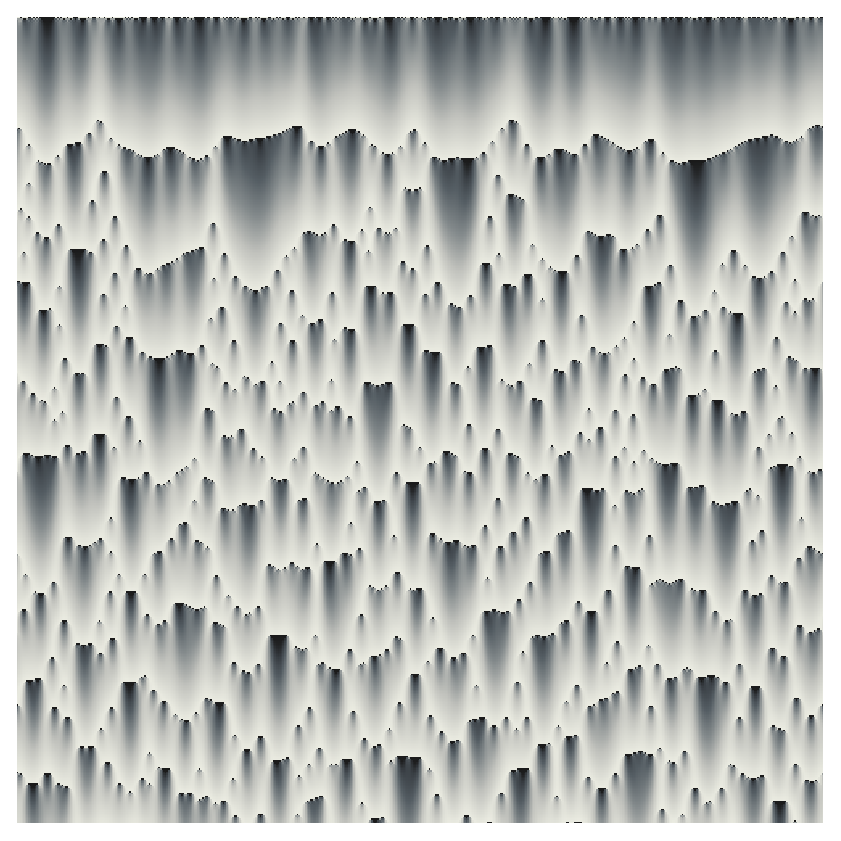
\includegraphics[width=.6\textwidth]{images/1d_cont_ca.png}
  \caption{Antonio Rueda Toicen}
\end{figure}
\end{frame}

\begin{frame}[c]\frametitle{Algol}
\begin{figure}
  \centering
  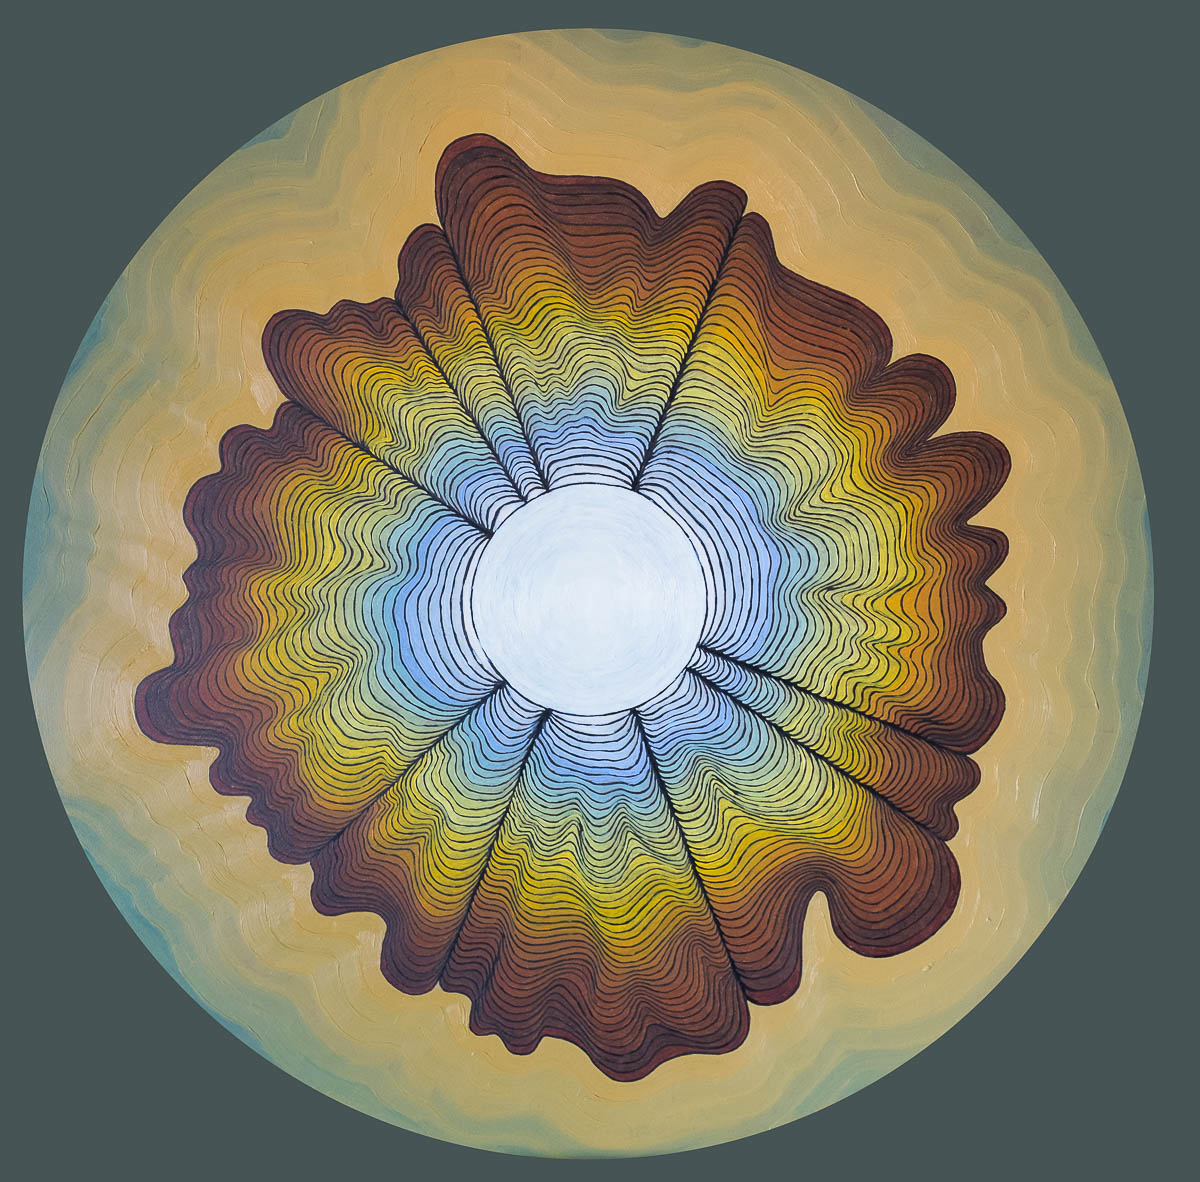
\includegraphics[width=.6\textwidth]{images/algol.jpg}
  \caption{Micky. 50x50, Oil color on board, 2016}
\end{figure}
\end{frame}

\begin{frame}[c]\frametitle{Concept/proposal}
\large
\begin{itemize}
  \item Combine regular plotting with optical feedback
  \item Give the robot some degree of freedom %using rules/algorithms
  \item Robot can extrapolate or improvise %when given direction
\end{itemize}

% Drowbot combines a regular plotting machine with optical feedback.
% We can utilize rules or algorithm to give the robot some degree of freedom.
% This way the robot can extrapolate or improvise upon the direction given by the artist.


\end{frame}

\begin{frame}[c]\frametitle{Example: CNC Drawing Robot}
\begin{figure}
  \centering
  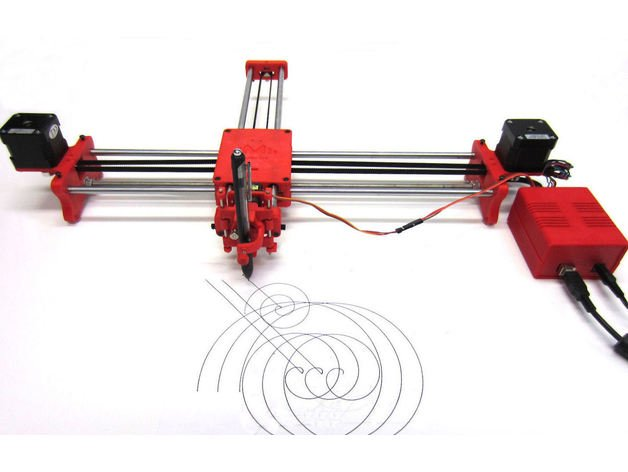
\includegraphics[width=.7\textwidth]{images/drawingrobot1.jpg}
  \caption{Henry Arnold, on Thingyverse.com}
\end{figure}
\end{frame}

\begin{frame}[c]\frametitle{Example: Drawing Arm}
\begin{figure}
  \centering
  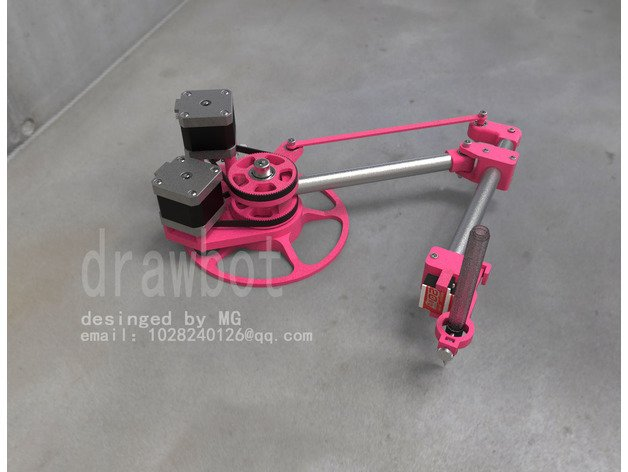
\includegraphics[width=.7\textwidth]{images/drawingrobot2.jpg}
  \caption{Ming Zhang, on Thingyverse.com}
\end{figure}
\end{frame}

\begin{frame}[c]\frametitle{Example: Drawing Robot}
\begin{figure}
  \centering
  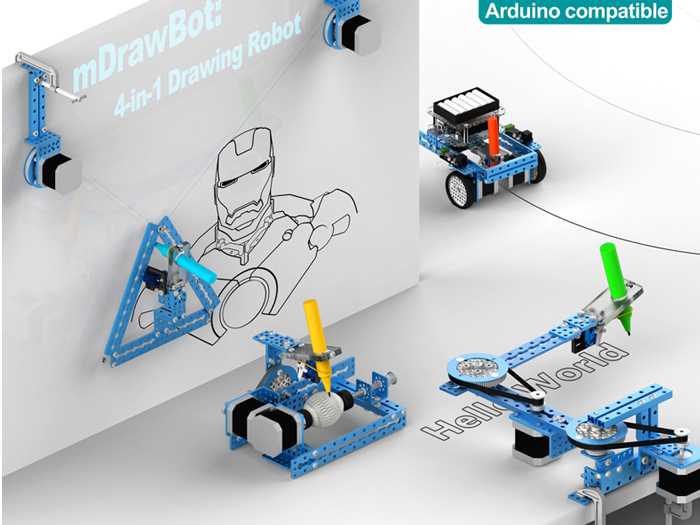
\includegraphics[width=.7\textwidth]{images/drawingrobot3.jpg}
  \caption{Makeblock mDrawBot}
\end{figure}
\end{frame}

\begin{frame}[c]\frametitle{Example: Vertical CNC}
\begin{figure}
  \centering
  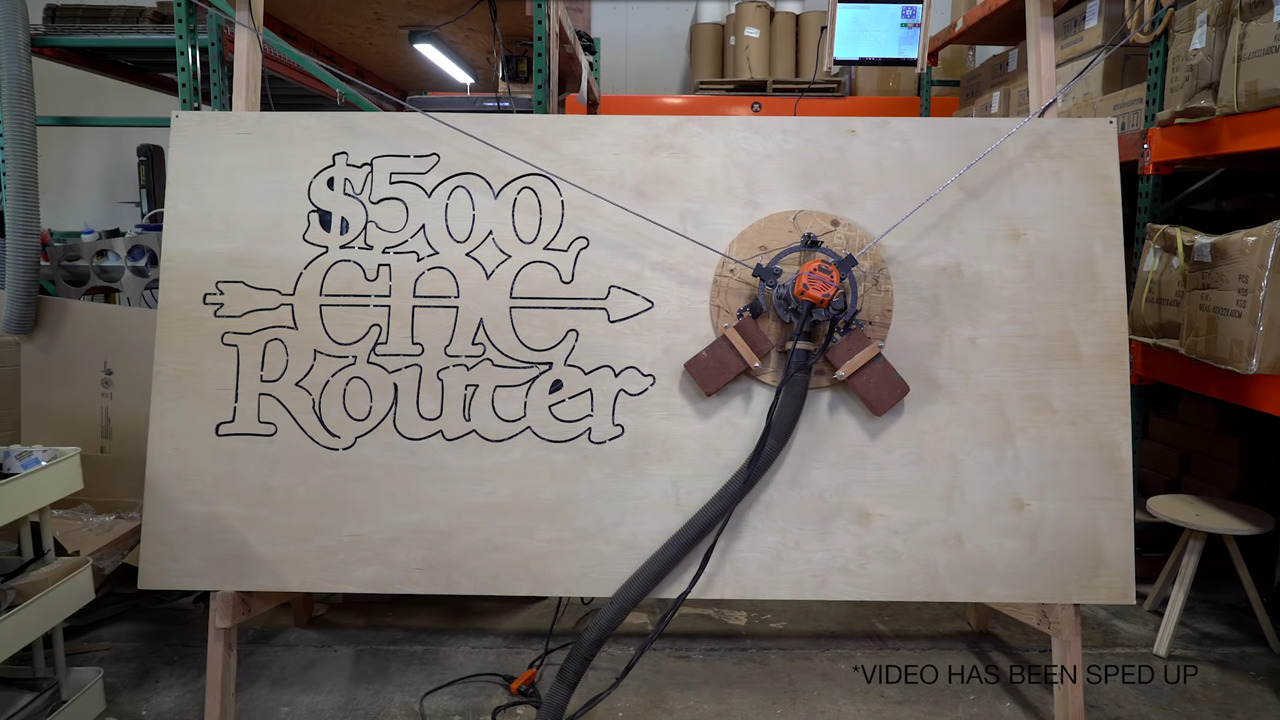
\includegraphics[width=.8\textwidth]{images/maslowCNC.jpg}
  \caption{Maslow CNC}
\end{figure}
\end{frame}


\begin{frame}[c]\frametitle{Goal}
\large
\begin{itemize}
  \item Find the most suitable architecture
  \item Build a simple proof-of-concept
  \item Experiment with different rules or algorithms
  \item Operate the robot directly on the blackboard
\end{itemize}
\end{frame}


\end{document}